% Auto-generated by scripts/build_eval_figures.py — do not edit.
\begin{figure}[t]
  \centering
  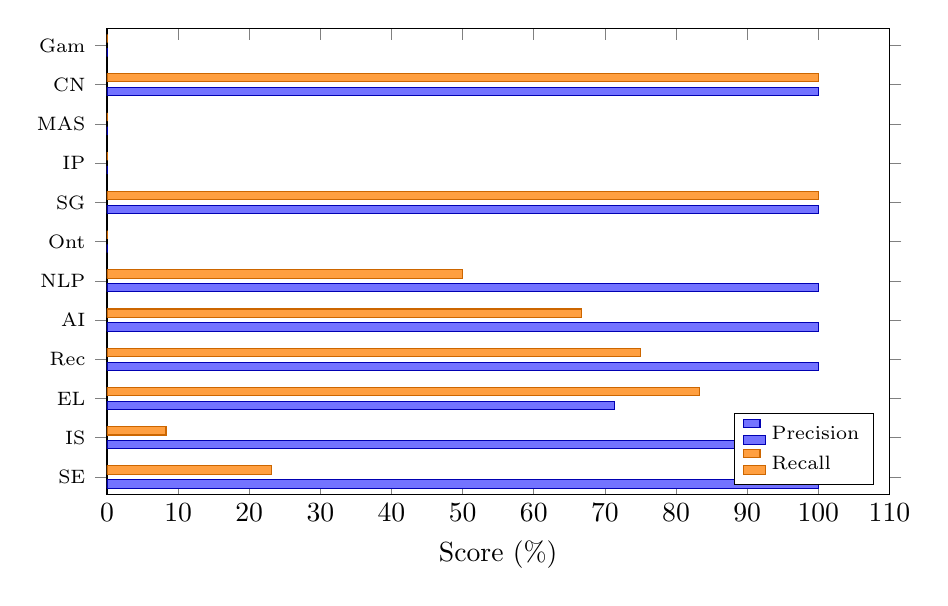
\begin{tikzpicture}
    \begin{axis}[
      width=0.95\linewidth, height=7.5cm,
      xbar, xmin=0, xmax=110,
      bar width=3pt, enlarge y limits=0.04,
      xlabel={Score (\%)},
      ytick={0,1,2,3,4,5,6,7,8,9,10,11},
      yticklabels={SE,IS,EL,Rec,AI,NLP,Ont,SG,IP,MAS,CN,Gam},
      yticklabel style={font=\scriptsize},
      legend style={font=\scriptsize,at={(0.98,0.02)},anchor=south east},
      legend cell align=left,
      ]
      \addplot+[fill=blue!55,draw=blue!70!black] coordinates {(100.0,0) (100.0,1) (71.4,2) (100.0,3) (100.0,4) (100.0,5) (0.0,6) (100.0,7) (0.0,8) (0.0,9) (100.0,10) (0.0,11)}; \addlegendentry{Precision}
      \addplot+[fill=orange!75,draw=orange!80!black] coordinates {(23.1,0) (8.3,1) (83.3,2) (75.0,3) (66.7,4) (50.0,5) (0.0,6) (100.0,7) (0.0,8) (0.0,9) (100.0,10) (0.0,11)}; \addlegendentry{Recall}
    \end{axis}
  \end{tikzpicture}
  \caption{Per-class precision and recall of \texttt{qwen2.5:14b-instruct} on the gold set. Classes for which precision is high but recall is low ({IS}, {SE}) are gold parents that the model legitimately splits into more specific {IEEE} children, the granularity gap discussed in \cref{sec:res-o1}.}
  \label{fig:precision-recall-gap}
\end{figure}
